\documentclass[../main.tex]{subfiles}
\graphicspath{{\subfix{../diagrams/}}}

\begin{document}

\chapter{Functional Verification}

\section{Introduction}
The purpose of functional verification is to ensure that the design meets the set specifications and that it can perform according to the requirements.\\
\newline
With the rapid developments in integrated circuit manufacturing technologies and the advances in computer aided design and design automation, integrated circuits are becoming more and more complex and large-scale than before. Although design time can be shortened by using modern CAD tools, verification time grows exponentially for SoC and microprocessors. Under time-to-market pressure, the verification requirements of are much tougher. Verification of complex systems has become one of the major bottlenecks in the development of SoC and computing systems. The methods of pure directed testing is not adaptive to the verification of modern day designs, because it is very time-consuming to write all test programs manually. Thereby, it is necessary to adapt more advanced methodologies to speed up the verification process. Many methodologies have been presented, such as open verification methodology (OVM), verification methodology manual (VMM) and Universal verification Methodology (UVM).\cite{Spear}

\section{The UVM}
The universal verification methodology is the latest endeavour of creating a unified verification environment.
It combines the efforts of the VMM and OVM into a true industry-wide methodology. \\
\newline
It is based on the the hardware design and verification language, SystemVerilog. Bringing the OOP concepts of software to hardware verification, it enabled the the opportunity of reusability and modularity of test components for a veriety of designs.\\
The UVM class library provides the building blocks needed to develop reliable and reusable verification components and test environments in SystemVerilog. In essence, UVM provides a set of classes, including plenty of methods for users to inherit and reuse. It also provides base class utilities and macros for managing log files and inter-process communication. Figure \ref{fig:uvm_testbench} shows a typical UVM diagram.

%%adding figure
\begin{figure}[h!]
\centering
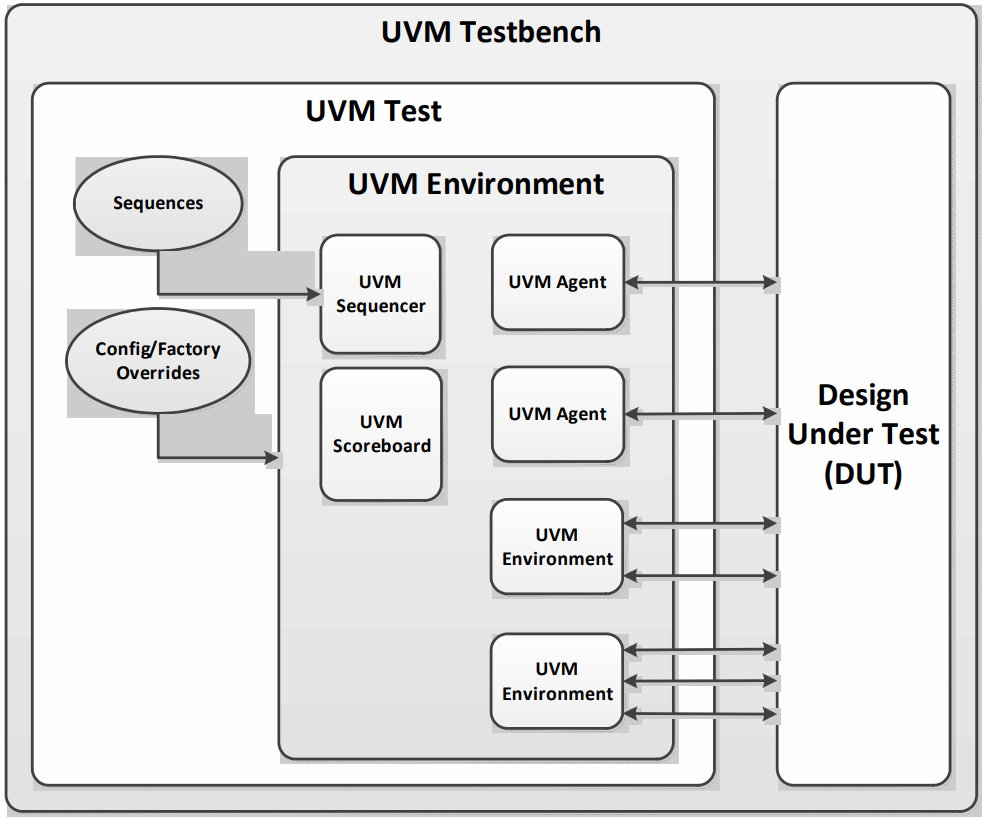
\includegraphics[scale = 0.4]{diagrams/UVM_testbench.png}
\caption{Typical UVM testbench architecture\cite{accelera}}
\label{fig:uvm_testbench}
\end{figure}

\subsection{The UVM hierarchy}
The UVM class hierarchy starts from the uvm\_object class, this class is the parent from which all other classes of the library are extended. 

\begin{itemize}
  
\item \textbf{UVM Test:}\\
The UVM Test is the top-level UVM Component in the UVM testbench. The UVM Test typically performs
three main functions:

\begin{enumerate}
    \item Instantiates the top-level environment
    \item Configures the environment (via factory overrides or the configuration database)
    \item Applies stimulus by invoking UVM Sequences through the environment to the DUT.
\end{enumerate}

Typically, there is one base UVM Test with the UVM Environment instantiation and other common items. Other individual tests will extend this base test and configure the environment differently or select different sequences to run.

\item \textbf{UVM Environment:}\\
The UVM Environment is a hierarchical component that groups together other verification components that
are interrelated. Typical components that are usually instantiated inside the UVM Environment are UVM
Agents, UVM Scoreboards, or even other UVM Environments. 
The top-level UVM Environment encapsulates all the verification components targeting the DUT.

\item \textbf{UVM Scoreboard:}\\
The UVM Scoreboard’s main function is to check the behavior of a certain DUT. The UVM Scoreboard
usually receives transactions carrying inputs and outputs of the DUT through UVM Agent analysis ports, runs the input transactions through a reference model or a checker to produce expected transactions, and then compares the expected
output versus the actual output.
There are different methodologies on how to implement the scoreboard, the nature of the reference model,
and how to communicate between the scoreboard and the rest of the testbench.

\item \textbf{UVM Agent:}\\
The UVM Agent is a hierarchical component that groups together other verification components that are
dealing with a specific DUT interface. A typical UVM Agent includes a UVM Sequencer to
manage stimulus flow, a UVM Driver to apply stimulus on the DUT interface, and a UVM Monitor to monitor the DUT interface. UVM Agents might include other components, like coverage collectors, protocol checkers, a TLM model, etc.

\begin{figure}[h!]
\centering
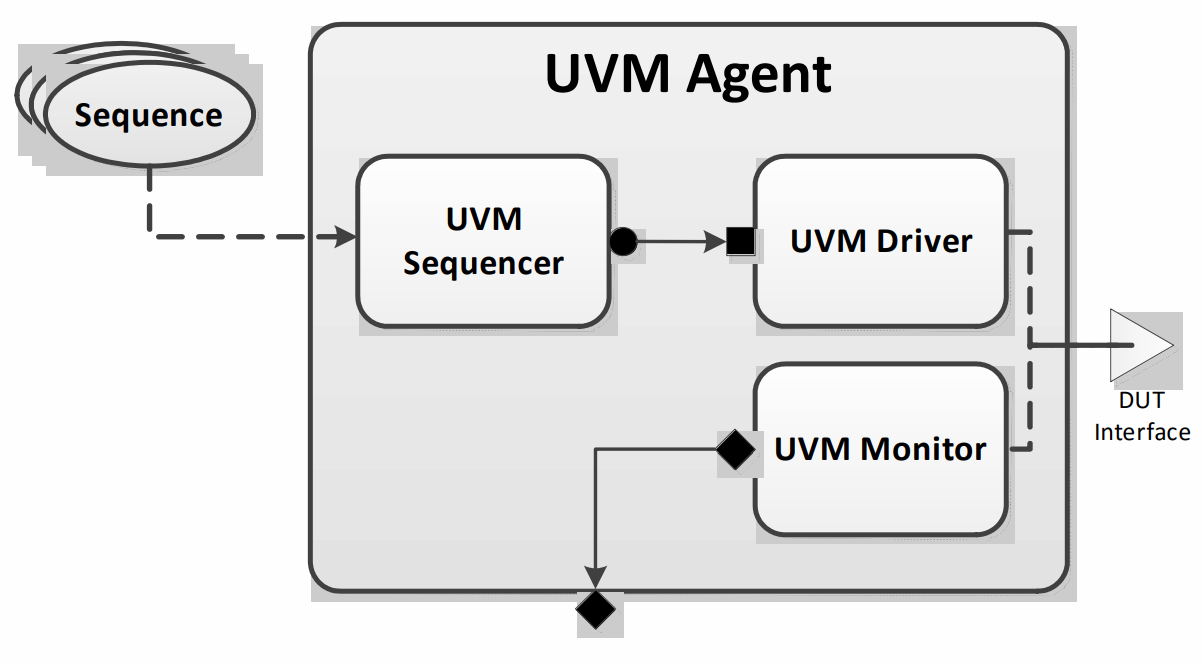
\includegraphics[scale = 0.4]{diagrams/UVM_agent.png}
\caption{UVM agent\cite{accelera}}
\label{fig:uvm_agent}
\end{figure}

The UVM Agent can operate in two modes: an active mode (where it is capable of generating stimulus), and a
passive mode (where it only monitors the interface without controlling it).

\item \textbf{UVM Sequencer:} \\
The UVM Sequencer controls the flow of UVM Sequence Items transactions generated by
one or more UVM Sequences. It is an arbiter for controlling and managing multiple sequences

\item \textbf{UVM Sequence:} \\
A UVM Sequence is an object that contains a behavior for generating stimulus. UVM Sequences are not part
of the component hierarchy. 

\item \textbf{UVM Driver:}\\ 
The UVM Driver receives individual UVM Sequence Item transactions from the UVM Sequencer and
applies (drives) it on the DUT Interface. Thus, a UVM Driver spans abstraction levels by converting
transaction-level stimulus into pin-level stimulus. It also has a TLM port to receive transactions from the
Sequencer and access to the DUT interface in order to drive the signals.

\item \textbf{UVM Monitor:}\\
The UVM Monitor samples the DUT interface and captures the information there in transactions that are
sent out to the rest of the UVM Testbench for further analysis. Thus, similar to the UVM Driver, it spans
abstraction levels by converting pin-level activity to transactions. In order to achieve that, the UVM Monitor
typically has access to the DUT interface and also has a TLM analysis port to broadcast the created
transactions through.
\end{itemize}

\begin{figure}[h!]
\centering
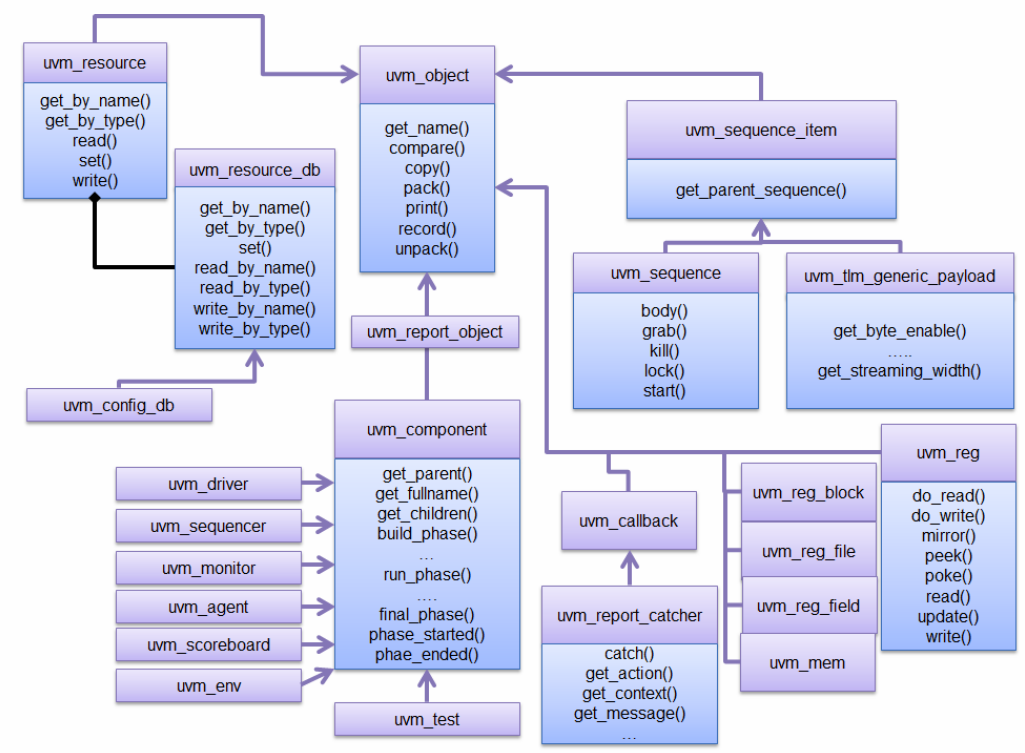
\includegraphics[scale = 0.6]{diagrams/UVM_hirearchy.png}

\caption{UVM hierarchy\cite{accelera}}
\label{fig:uvm_hierarchy}
\end{figure}

\subsection{UVM phases}
 UVM phases are the set of functions and tasks that all UVM components execute together. All UVM components are always synchronized with respect to these phases.\\
The phases are executed in the following sequence. See figure \ref{fig:uvm_phase}.\\
\begin{itemize}
\item \textbf{build\_phase:} Creates and configures the testbench structure.
\item \textbf {connect\_phase:} Establishes cross-component connections.
\item \textbf {end\_of\_elaboration\_phase:} Displays UVM topology and other functions required to be done after connection.
\item \textbf {start\_of\_simulation\_phase:} Sets initial run-time configuration or display topology.
\item \textbf {run\_phase:} The actual simulation that consumes time happens in this UVM phase and runs in parallel to other UVM run-time phases.
\item \textbf {extract\_phase:} Extracts data from different points of the verification environment.
\item \textbf {check\_phase:} Performs scoreboard tasks that checks for errors between expected and actual values from design.
\item \textbf {report\_phase:} displays result from checkers, or summary of other test objectives.
\item \textbf {final\_phase:} does last minute operations before exiting the simulation.
\end{itemize}
%% add figure
 \begin{figure}[h!]
\centering
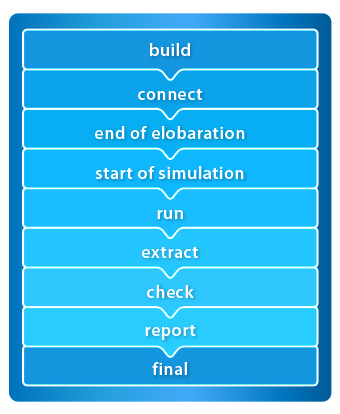
\includegraphics[scale = 0.8]{diagrams/uvm_phase_01.jpg}
\caption{UVM phases}
\label{fig:uvm_phase}
\end{figure}

 \noindent All UVM phases follow the bottom up approach except for the build\_phase and final\_phase, they are executed in a top-down fashion.\newline
 All UVM phases are functions except for the run\_phase which is a task.
 
\section{RISC-V Verification}
Processor verification is a much more complex task than SOC verification. As SOC verification is focused on verifying the connection of interfaces between the different IPs and the integration of the different modules, processor verification is focused on the correct implementation of the core; is it to the standard specification, are instructions being executed correctly, are the miscellaneous variations of instruction sequences are executed correctly or do they cause a deadlock in the execution flow? All these questions and more are vital when verifying the processor.\\
\newline
To verify a processor, six key components are required:\cite{StepCompare}  
\begin{enumerate}
\item The DV plan (coverage metrics, debug modes, asynchronous events, etc).
\item RISC-V processor RTL implementation as the Device Under Test (DUT).
\item SystemVerilog testbench IP with supporting infrastructure and interfaces.
\item Selection of test suites and generators, including directed, random, and compliance tests.
\item Reference model to compare against the same tests running on the DUT.
\item Simulation environment.
\end{enumerate}

\subsection{Reference models}
The complexity of the processors makes it hard to check for the correctness of the results produced by the processor. To overcome this issue, the processor under test is compared against another reference processor. This reference processor is written in a higher-level language like C or python. It can be used as an instruction set simulator (ISS) for software development or a reference model. It should also have gone under an extensive amount of testing to ensure that it is a valid model, we do not want a faulty reference model. The RISC-V architecture has a wide range of supported reference models. Four models where models were selected as viable candidates (table \ref{UVM.ISS}).\\
\newline
\noindent The metrics of selecting a viable model are as followed:
\begin{itemize}
    \item Is the ISS open-source?
    \item Does it support the full ISA?
    \item Is it well documented for both simulation and verification?
    \item Does it support integration with a UVM environment?
\end{itemize}

\noindent Out of the four models and using the previously mentioned metrics, one model was selected. Table \ref{UVM.ISS} shows a comparison between the features of the four models.
\newpage

\begin{table}[h!]
\begin{center}
\begin{tabular}{p{3cm} | p{2.8cm} | p{2.5cm} | p{1.5cm} | p{2.7cm} |}
    & \textbf{Spike}&\textbf{Whisper} & \textbf{Sail} & \textbf{OVPsimPlus}\\
    \hline
    \textbf{Open Source}& Yes& Yes & Yes & Yes\\ 
    \hline
	\textbf{Full ISA Support}& Yes& No S/U modes & Yes & Yes\\
	\hline
	\textbf{Documented for testing}& No& No & Yes & Yes\\
	\hline
	\textbf{UVM support} & Requires modifications& Yes & Yes & Yes\\
	\hline
	\textbf{Used by}& Ariane, Ibex, OpenHW group & SweRV cores & NA & OpenHW group\\
	\hline
\end{tabular}
\end{center}
\caption{RISC-V instruction set simulators }
\label{UVM.ISS}
\end{table}

\noindent riscvOVPsimPlus is free and opensource version. A commercial version with additional features is also available. Sail also has a random instruction generator.


\subsection{The Google RISCV-DV}
It is an open-source instruction generator developed by Google for RISC-V processor verification based on SV/UVM. It has been verified with various simulators.\\
The following four concepts are the pillars for RISCV-DV:
\begin{enumerate}
\item \textbf{Randomness:} There are three levels of randomization
\begin{itemize}
    \item Instruction level randomization:\\
  Cover all possible operands and immediate values of each instruction.
   \item  Sequence level randomization:\\
   The instruction generator should Maximize the possibility of instruction orders and dependencies.
   \item Program level randomization:\\
     Random privileged mode setting, page table organization, program calls.
\end{itemize}
\item \textbf{Architecture-aware:} The generated program should be able to hit the corner cases of the processor architectural features.
\item \textbf{Performance:} The instruction generator should be scalable to generate a large program in a short time.
\item \textbf{Extendability:} Easy to add new instruction sequences, custom instruction extension, custom CSR, etc.
\end{enumerate}

 \noindent RISCV-DV currently supports the following features:

\begin{itemize}
\item 	Supported instruction set: RV32IMAFDC, RV64IMAFDC.
\item 	Supported privileged mode: machine mode, supervisor mode, user mode.
\item 	Page table randomization and exception.
\item 	Privileged CSR setup randomization.
\item 	Trap/interrupt handling.
\item 	Sub-program generation and random program calls.
\item 	Illegal instruction and HINT instruction generation.
\item 	Random forward/backward branch instructions.
\end{itemize}

\subsection{Step-and-Compare verification}
In a step/compare simulation environment the basic approach is to compare the same input stimulus to both the RTL (DUT) against the reference model. Meaning that after every instruction execution the simulation is paused, and the log from both the DUT and the reference model are compared against each other. \\
\newline
\noindent While this may be supported with a log file comparison approach, it does not meet requirements around debug operations and asynchronous events. 

\noindent Figure \ref{fig:Stepcompare1} illustrates the approach known as the ‘step-and-compare’ method, which directly synchronizes the DUT and the reference model at every instruction retirement.

\noindent Figure \ref{fig:Stepcompare2} illustrates the connection method between the DUT and the ISS.

\begin{figure}[h!]
\centering
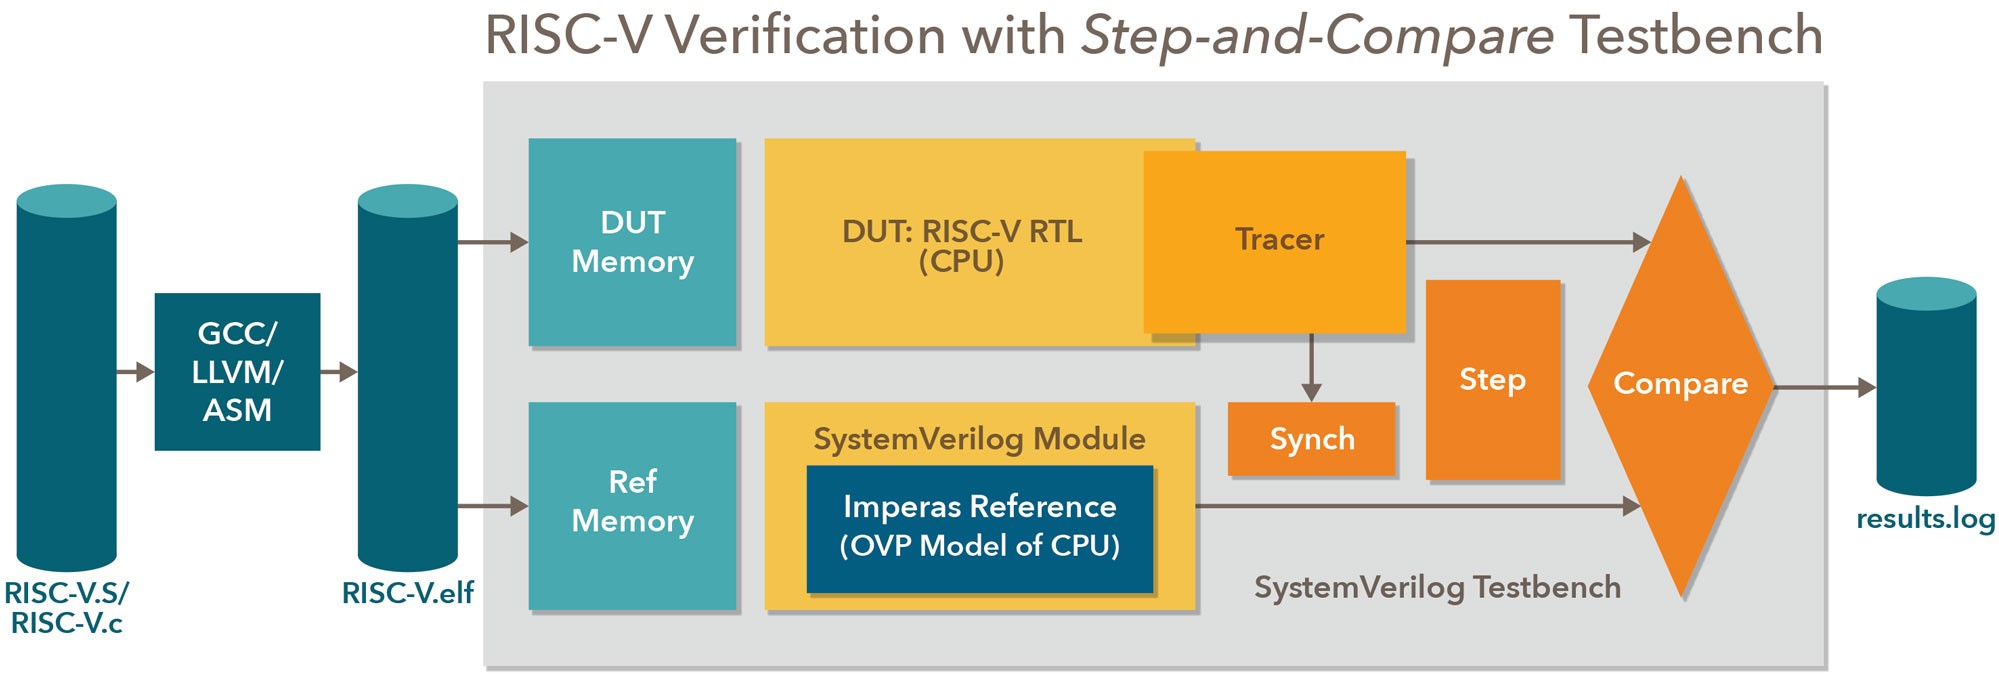
\includegraphics[scale = 0.3]{diagrams/step_compare1.jpg}

\caption{Verification environment in the step-and-compare flow\cite{StepCompare}}
\label{fig:Stepcompare1}
\end{figure}

\begin{figure}[h!]
\centering
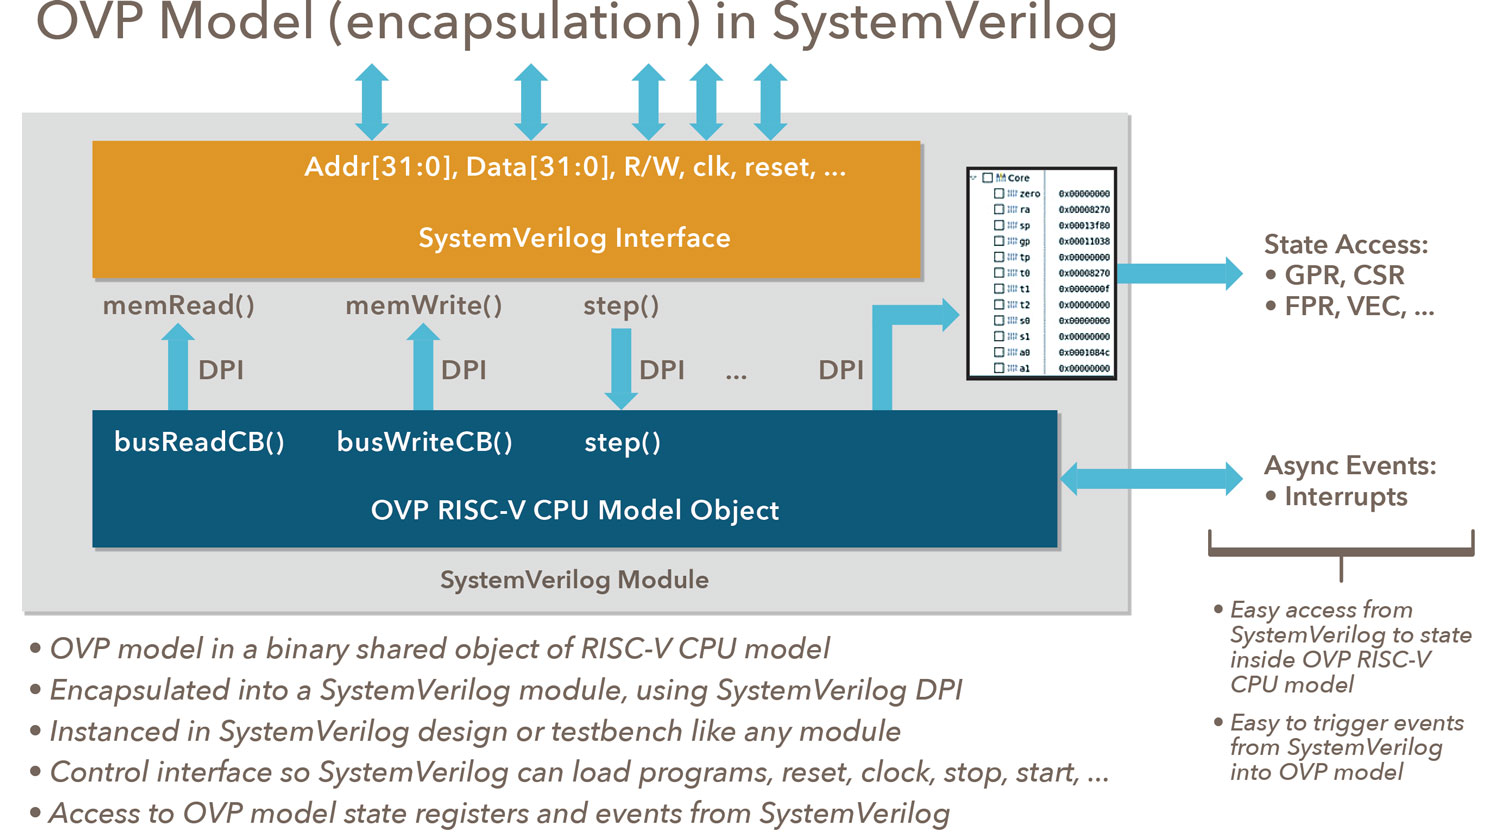
\includegraphics[scale = 0.3]{diagrams/step_compare2.jpg}

\caption{Connection between the RTL DUT and the reference model in a step/compare flow\cite{StepCompare}}
\label{fig:Stepcompare2}
\end{figure}

\section{Processor Verification}
\subsection{Memory model}
To run the large amounts of assembly instructions on an RTL based processor, a memory is required. Simulating the whole 4GB memory would be inefficient and resources consuming. An alternative method is to use a c language based memory or a UVM based one. This way the memory is allocated to the processor only when it is in use, making the simulation faster and more efficient.\\
\newline
\noindent For this case, we architected a UVM based memory model. The model we propose is transaction level based making it independent of the memory interface. It also allows it to be used in verification of other processors or any system the requires large amounts of memory.\\
\newline
\noindent Figure \ref{fig:UVM_memory} illustrates the architecture of the memory agent. The memory agent consists of the following:

\begin{figure}[h!]
\centering
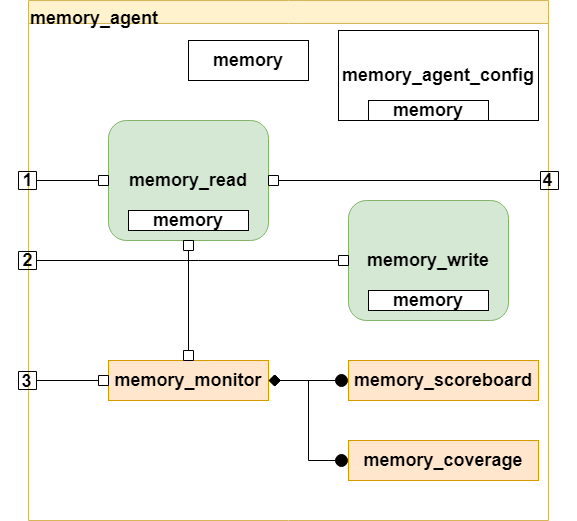
\includegraphics[scale = 0.5]{diagrams/UVM_Memory_Model.png}

\caption{Architecture of the verification memory model}
\label{fig:UVM_memory}
\end{figure}

\begin{itemize}
\item 	\textbf{memory:}\\
The memory is a UVM object class with an associative array that represents the system memory and some methods and macros for operating on the array.
\item 	\textbf{memory\_read:}\\
The memory read is a UVM driver class. It is responsible for receiving and responding to memory read requests.\\
It has two ports; the get port receives memory read requests from the processor, and the put port sends the the read responses back to the processor.
\item 	\textbf{memory\_write:}\\
The memory write is also a UVM driver class. It is responsible for receiving and executing write requests to the memory.\\
It has a single get port that receives memory write requests.
\item 	\textbf{memory\_monitor:}\\
The monitor is a UVM monitor class. It is responsible for generating the memory log file and extracting the memory contents at the end of simulation.\\
It has a single get port that receives both read and write requests for logging.
It also has a single analysis port that is connected to both coverage and scoreboard objects.
\item 	\textbf{memory\_scoreboard:}\\
The scoreboard is UVM scoreboard class. It check if each request and response are executed correctly.
\item 	\textbf{memory\_coverage:}\\
The coverage class keeps track of the memory addresses which have been written to and read from during the simulation.
\item 	\textbf{memory\_agent\_config:}\\
The agent configuration object configures the memory and memory agent according to simulation requirements.
\end{itemize}

\subsection{Core agent}
\begin{figure}[h!]
\centering
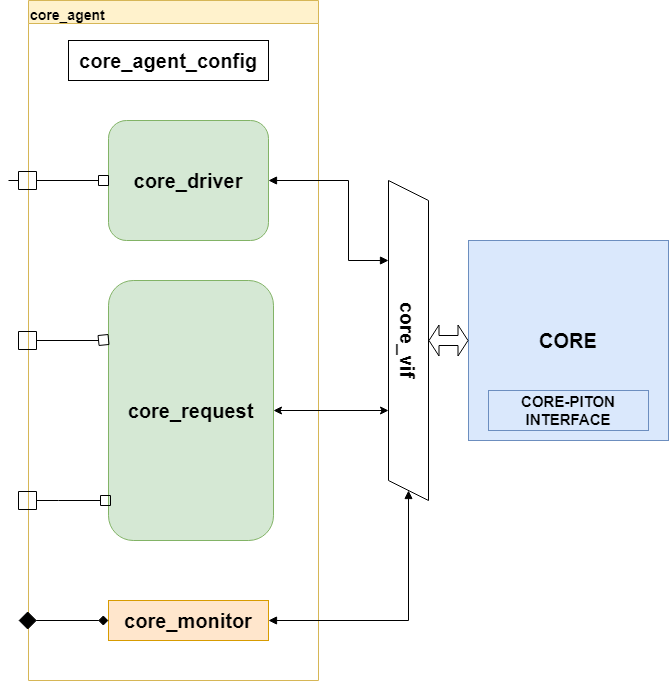
\includegraphics[scale = 0.5]{diagrams/UVM_CORE_AGENT.png}

\caption{Core agent}
\label{fig:UVM_core}
\end{figure}

\begin{itemize}
\item 	\textbf{core\_driver:}\\
The driver is a UVM driver class that is connected to the core by the core interface. It is responsible for converting read response transaction to  signals. It is also used for asserting any other inputs to the core.
\item 	\textbf{core\_request:}\\
The core read request is a UVM driver class. It wraps the core request signals into a transaction class.
\item 	\textbf{core\_monitor:}\\
The core monitor creates the core log. That is after each instruction execution it stores the values of privileged and unprivileged registers, the program counter. It also stores the outgoing and in-going requests.
\item 	\textbf{core\_agent\_config:}\\
The agent configuration object configures agent according to simulation requirements. It also contains the handle to the core interface.
\end{itemize}

\subsection{UVM environment}
The Complete UVM environment is illustrated in figure \ref{fig:UVM_env}. It is structured as follows:

\begin{itemize}
\item 	\textbf{top:}\\
This is the top module has the folowing tasks:
\begin{enumerate}
    \item Instantiate the DUT.
    \item Connect the virtual interface and passes it down to the UVM objects.
    \item Declare the test class.
    \item Run the tests.
\end{enumerate}
\item 	\textbf{core\_test:}\\
It is a UVM test class. It wraps the core\_env class and runs the required tests.
\item 	\textbf{core\_env:}\\
It is a UVM environment. It instantiates the core agents and makes the required connections using ports and FIFOs.
\end{itemize}

\begin{figure}[p]
\centering
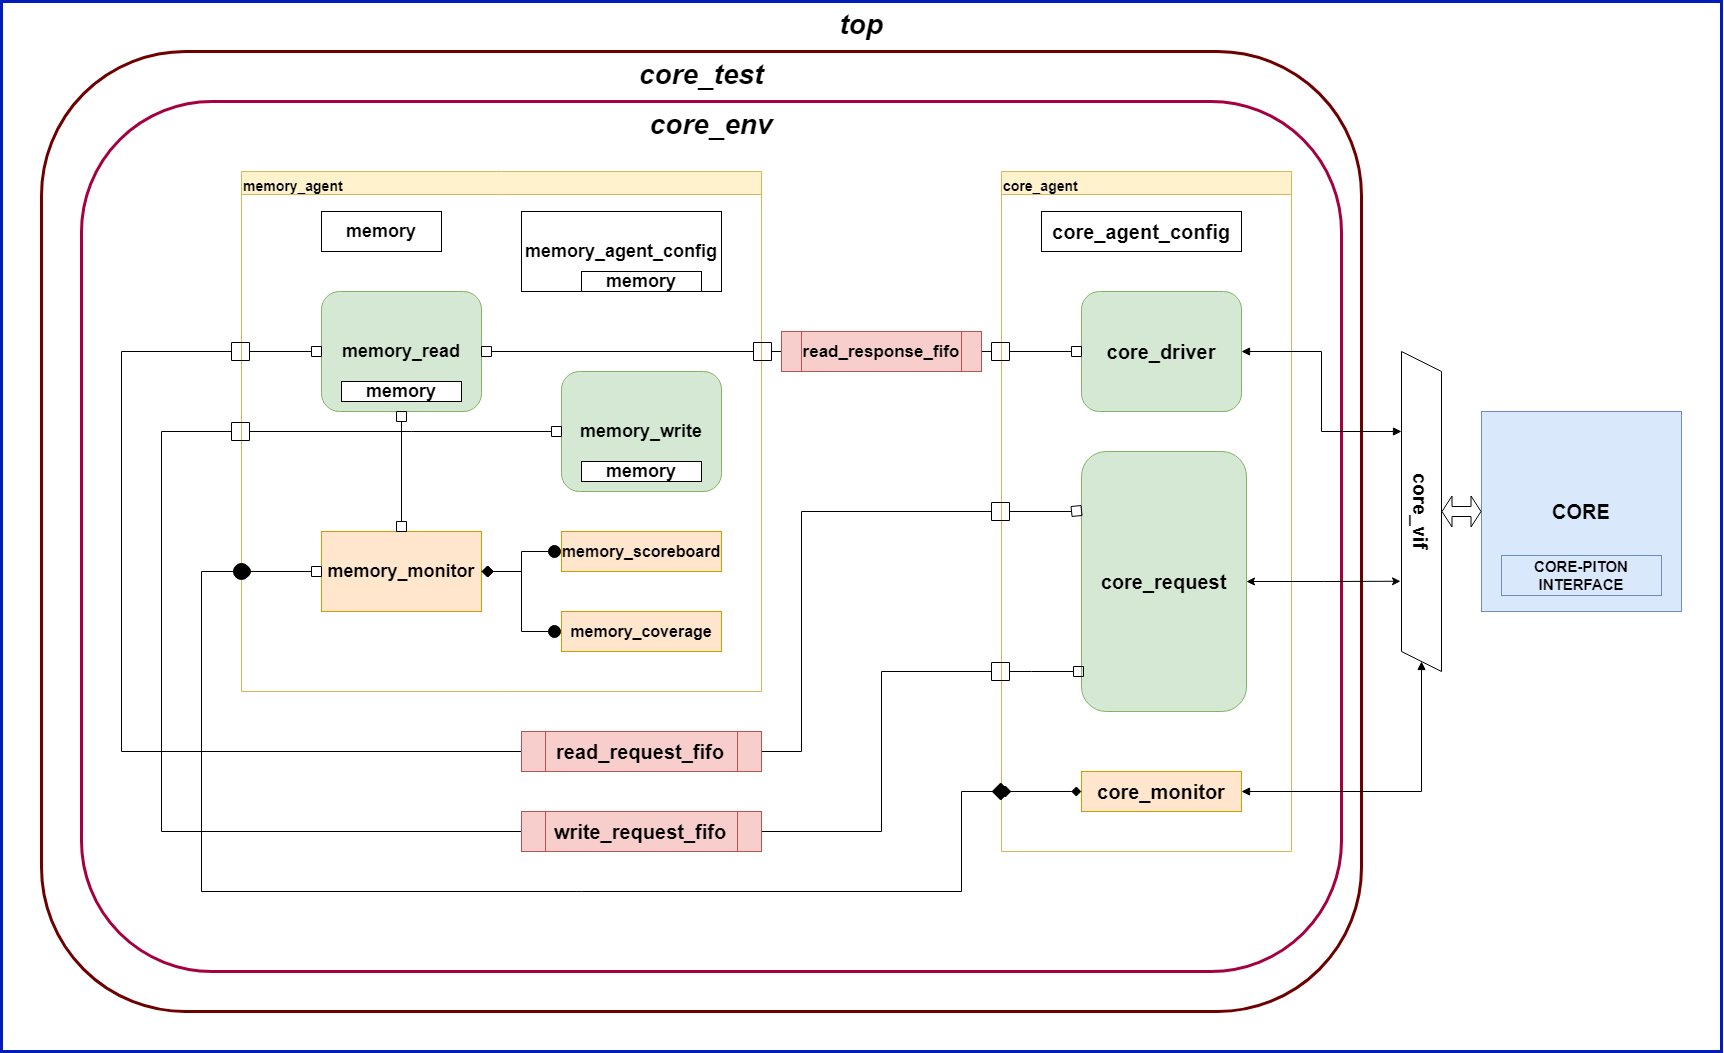
\includegraphics[scale = 0.38, angle = 90]{diagrams/UVM_CORE_ENVIRONMENT.png}

\caption{Complete UVM environment}
\label{fig:UVM_env}
\end{figure}

\newpage
\subsection{Verification flow}
While a step-and-compare flow is more advisable; as it combines the whole simulation components in a unified environment, just-in-time debugging, full utilization of UVM components, but a we preferred to use a trace and compare approach to achieve faster development time, and easier logging and log comparisons using friendlier software languages such as python.\\

\noindent In a trace-and-compare flow, the simulation and logging of the reference model and the DUT are carried out separately and the log comparison is done post simulation.\\

\noindent The flow is as illustrated in figure \ref{fig:UVM_flow}. It consists of mainly five steps:
\begin{enumerate}
    \item Random instruction generation: For this step we used RISCV-DV.
    \item Compilation: The open-source RISCV tool-chain is used to generate the elf binary and hex files for the reference model and the DUT respectively.
    \item Simulation: The resulting file from the previous step are loaded into their respective targets and the simulation is carried out.
    \item Log comparison and reporting: The resulting log files are compared against each other and any anomalies are reported.
    \item Debugging: In this step, the bugs are traced back and corrected.
\end{enumerate}

\begin{figure}[h!]
\centering
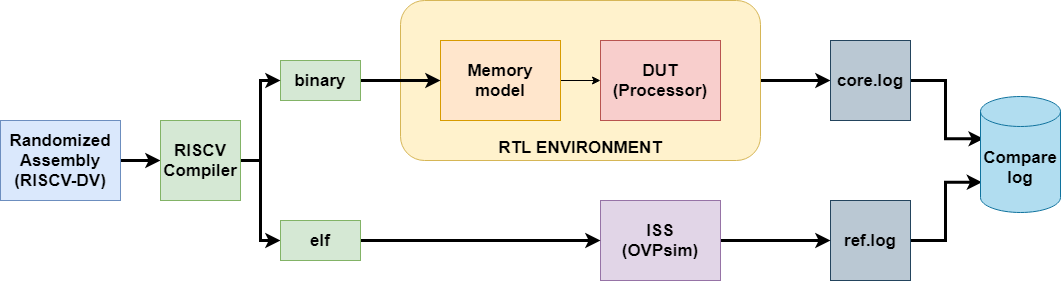
\includegraphics[scale = 0.4]{diagrams/UVM_FLOW.png}

\caption{Processor verification flow}
\label{fig:UVM_flow}
\end{figure}

\section{Verification Results}
\end{document}
